\documentclass[a4paper,9pt,oneside]{scrreprt}
\usepackage[latin1]{inputenc}
\usepackage[T1]{fontenc}
\usepackage{ae,aecompl}
\usepackage[english]{babel}
\usepackage{amsmath}
\usepackage{amssymb}
\usepackage{amsfonts}
\usepackage{amsthm}
\usepackage{graphicx}
\usepackage{wrapfig}
\usepackage{ulem}
\usepackage{cancel}
\usepackage{float}
\usepackage{color}
\usepackage{titlesec}
\usepackage{geometry}
\geometry{verbose,a4paper,tmargin=25mm,bmargin=25mm,lmargin=15mm,rmargin=25mm}
\titlelabel{\thetitle.\quad}
\usepackage{tabularx}
\usepackage{booktabs}
\usepackage{paralist}
\usepackage{textcomp}

\usepackage{graphicx}
\usepackage{paracol}


\renewcommand{\rmdefault}{phv}
\renewcommand{\sfdefault}{phv}

\usepackage{color}

\definecolor{pblue}{rgb}{0.13,0.13,1}
\definecolor{pgreen}{rgb}{0,0.5,0}
\definecolor{pred}{rgb}{0.9,0,0}
\definecolor{pgrey}{rgb}{0.46,0.45,0.48}

\usepackage{listings}
%\lstset{
%	numbers=left,
%	breaklines=true,
%	tabsize=2,
%	literate={\ \ }{{\ }}1,
%	language=Java,
%	basicstyle=\footnotesize\ttfamily, 
%	stepnumber=1,
%	%	aboveskip=-10pt,
%}

\lstset{language=Java,
	tabsize=2,
	showspaces=false,
	showtabs=false,
	breaklines=true,
	showstringspaces=false,
	breakatwhitespace=true,
	commentstyle=\color{pgreen},
	keywordstyle=\color{pblue},
	stringstyle=\color{pred},
	basicstyle=\footnotesize\ttfamily,
	moredelim=[il][\textcolor{pgrey}]{$$},
	moredelim=[is][\textcolor{pgrey}]{\%\%}{\%\%}
}


\begin{document}
\begin{tabular}{ccc}
	\begin{large} \textbf{Prof. Lichter} \end{large} &
	
	\begin{minipage}[H]{3.5cm}
	\centering
		\begin{large} OOSC \end{large} \\
		\begin{large} WS 2016/2017 \end{large}
	\end{minipage} &
	
	\begin{minipage}[H]{4cm}
%		\includegraphics[keepaspectratio,width=\textwidth,angle=0]{logoswc.png}
	\end{minipage} \\
Andreas Steffens, Konrad F\"ogen &  &  \\
& \begin{huge} \textbf{Submission 3} \end{huge}&  \\
& oosc@swc.rwth-aachen.de &  \\
& & \\
 % Hier drunter müssen die Daten noch angepasst werden
Issued: 21.05.2019 &
Submission: 04.06.2019 &
Discussion:  07.06.2019 \\
\end{tabular}
\newline \newline \newline

\begin{center}
	Submitted by Group 09
	
	\bigskip
	
	\begin{tabular}{ll}
		Ulfet CETIN & 391819 \\
		Saud KHAN & 392365  \\
		Samuel ROY & 391822 \\
		Charulekha, Besta Venkateswara RAO & 391844 \\
		Deepak SATEESH & 391813  \\
	\end{tabular}
	
	(ordered on lastname basis)
	
\end{center}


\setcounter{chapter}{3} % Aktuelles Assigment
	
\section{Task: Boundary-Value Analysis}
	\begin{enumerate}[a)]
		\item Please use the Boundary-Value Analysis to identify the input space. \\
		Please name all
necessary boundary values.
\\
		Create and implement a test suite with Junit5 using Boundary Value Testing.
		\bigskip
		
			Boundary values are given below for each variable:\\
			\begin{table}[H]
				\centering
				\begin{tabular}{|c|c|c|c|c|c|c|c|}
					
					\hline
					&&&&&&&\\
					Variable Name & min- & min & min+ & nom & max- & max & max+\\
					&&&&&&&\\
					\hline
					&&&&&&&\\
					local-part 	& 0 & 1 & 2 & 33 & 63 & 64 & 65 \\
					&&&&&&&\\
					\hline
					&&&&&&&\\
					domain-part & 0 & 1 & 2 & 65 & 127 & 128 & 129\\
					&&&&&&&\\
					\hline
					&&&&&&&\\
					top-part & 0 & 1 & 2 & 32 & 62 & 63 & 64\\
					&&&&&&&\\
					\hline
				\end{tabular}
				\bigskip
			
					* in case a during a nominal value calculation that an odd integer division  is \\
					encountered ( e.g. (128+1) / 2), we ceil the value to the nearest integer.\\
			\end{table}
		
			How values are determined:
			\begin{compactitem}
				\item range for length of each part of an e-mail is given in the assignment text,
				\begin{compactitem}
					\item  local part (local-part) $\Rightarrow$ [1,64]
					\item  domain part (domain-part) $\Rightarrow$ [1,128]
					\item  top-level domain (tld) $\Rightarrow$ [1,63]
				\end{compactitem}
			
				\item for min- and max-, I just decremented the respective value by 1,
				\item for min+ and max+, I just incremented the respective value by 1,
				\item for nominal value, I summed max and min together, and then divided the result by 2
			\end{compactitem}
			
			\clearpage
			\textbf{Simple Boundary Value Testing:}
		    
		    \begin{paracol}{2}
		    	
		    
%		    \renewcommand{\arraystretch}{1.8}
				\begin{table}[H]
					\scalebox{0.65}{
					\begin{tabular}{|c|c|c|c|c|c|c|c|}
						\hline
						Test Suite & Local  & Domain  & Top & email & Actual \\
						&	Length & Length & Length & Validator & Result\\
						\hline
						{[}Simple{]}&33&32&32& True & True \\
						\hline
						{[}Simple{]}&1&65&32& True & True \\
						\hline
						{[}Simple{]}&2&65&32& True & True \\
						\hline
						{[}Simple{]}&63&65&32& True & True \\
						\hline
						{[}Simple{]}&64&65&32& True & True \\
						\hline
						{[}Simple{]}&33&1&32& True & True \\
						\hline
						{[}Simple{]}&33&2&32& True & True \\
						\hline
						{[}Simple{]}&33&127&32& True & True \\
						\hline
						{[}Simple{]}&33&128&32& True & True \\
						\hline
						{[}Simple{]}&33&32&1& True & True \\
						\hline
						{[}Simple{]}&33&32&2& True & True \\
						\hline
						{[}Simple{]}&33&32&62& True & True \\
						\hline
						{[}Simple{]}&33&32&63& True & True \\
						\hline
					\end{tabular}
				}
					\bigskip
				\end{table}
			
			\switchcolumn
			
			We have 3 variables, and each has 5 values \{min, min+, nom, max-, max\} for simple BVT.\\
			How to run the test:			
			\begin{compactitem}
				\item for each variable in \{local, domain, top\}
					\begin{compactitem}
						\item for each \{min, min+, max-, max\} value of the variable
							\begin{compactitem}
								\item generate a test case with:\\
								(this variable's value from for,\\
								 other\_variable$_{nom}$, another\_variable$_{nom}$)
							\end{compactitem}
						
						\item do not forget to add the test case including all nominal values:
							\begin{compactitem}
								\item (variable$^{1}_{nom}$, variable$^{2}_{nom}$, variable$^{3}_{nom}$)
							\end{compactitem}
					\end{compactitem}
			\end{compactitem}
			\bigskip
						
		\end{paracol}
	
		This would lead to a total of (4*n + 1) test cases (4 different values for each variable, and 1 case consisting of all nominal values).\\
		
		Please note that the tests are generated using "@TestFactory" approach of JUnit 5, which allows for creating DynamicTest collections and providing them names for execution, easily allowing creating of separate test cases for combinations of values from variables.\\
		
		For generation of strings, I created functions that randomly generates strings from a character pool consisting of: \{ a to z, A to Z, 0 to 9  \}(endings inclusive). Another function generates triples of strings for test cases, given three of the lengths wanted. See the code below:
		
\begin{lstlisting}
	String characterPool = new String ("abcdefghijklmnopqrstuvwxyzABCDEFGHIJKLMNOPQRSTUVWXYZ0123456789");
	int characterPoolSize = characterPool.length();
	
	public String stringGeneratorbyLength(Random r, int stringLength) {
		if (stringLength == 0)
			return new String("");
	
		String resultString = new String("");
			for (int i=0; i<stringLength; i++) {
				int pickedValue = r.nextInt(characterPoolSize);
				resultString = resultString + characterPool.charAt(pickedValue);
			}
			return resultString;
	}
	
	public Triple<String, String, String> mailGeneratorByLength(Random r, int localLength, int domainLength, int topLength) {
		String _local = stringGeneratorbyLength(r, localLength);
		String _domain = stringGeneratorbyLength(r, domainLength);
		String _top = stringGeneratorbyLength(r, topLength);
		
		Triple<String, String, String> emailTriple = Triple.of(_local, _domain, _top);
		return emailTriple;
	}
\end{lstlisting}


		
	SimpleBVT test case generation part is the code below (for full code, please refer to the Appendix part of this document):
		
\begin{lstlisting}
@TestFactory
Collection<DynamicTest> simpleBVT() {
	List<Integer> localValues	= Arrays.asList( localMinLength, localMinLength_plus, localMaxLength_minus, localMaxLength);
	List<Integer> domainValues	= Arrays.asList( domainMinLength	, domainMinLength_plus	, domainMaxLength_minus	, domainMaxLength);
	List<Integer> topValues		= Arrays.asList( topMinLength, topMinLength_plus, topMaxLength_minus, topMaxLength);
	
	Random r = new Random();
	ArrayList<DynamicTest> tests = new ArrayList<DynamicTest>();
	
	for (Integer lVal: localValues) {
		Triple<String, String, String> s = mailGeneratorByLength(r, lVal, domainNomLength, topNomLength);
		DynamicTest t = DynamicTest.dynamicTest(testMessage,
			() -> Assertions.assertTrue(validator.validateEMailAdress(s.getLeft(), s.getMiddle(), s.getRight()), "pass"));
		tests.add(t);
	}
	/* similar for loops for domainValues and topValues is done, omitted from the document for shortness */
	
	return tests;
}
	
\end{lstlisting}
		
		
		
		\item Create and implement a test suite with Junit5 using Robustness BV Testing. Explain the
		changes and additions you made to the test suite.
		
				\textbf{Robustness Boundary Value Testing:}
			\begin{paracol}{2}
				
			
			\begin{table}[H]
				\scalebox{0.65}{
				\begin{tabular}{|c|c|c|c|c|c|c|c|}
					\hline
					Test Suite & Local  & Domain  & Top & email & Actual \\
					&	Length & Length & Length & Validator & Result\\
					\hline
					{[}Robustness{]}&33&32&32&true&true\\
					\hline
					{[}Robustness{]}&0&65&32&false&false\\
					\hline
					{[}Robustness{]}&1&65&32&true&true\\
					\hline
					{[}Robustness{]}&2&65&32&true&true\\
					\hline
					{[}Robustness{]}&63&65&32&true&true\\
					\hline
					{[}Robustness{]}&64&65&32&true&true\\
					\hline
					{[}Robustness{]}&65&65&32&false&false\\
					\hline
					{[}Robustness{]}&33&0&32&false&true\\
					\hline
					{[}Robustness{]}&33&1&32&true&true\\
					\hline
					{[}Robustness{]}&33&2&32&true&true\\
					\hline
					{[}Robustness{]}&33&127&32&true&true\\
					\hline
					{[}Robustness{]}&33&128&32&true&true\\
					\hline
					{[}Robustness{]}&33&129&32&false&false\\
					\hline
					{[}Robustness{]}&33&32&0&false&false\\
					\hline
					{[}Robustness{]}&33&32&1&true&true\\
					\hline
					{[}Robustness{]}&33&32&2&true&true\\
					\hline
					{[}Robustness{]}&33&32&62&true&true\\
					\hline
					{[}Robustness{]}&33&32&63&true&true\\
					\hline
					{[}Robustness{]}&33&32&64&false&false\\
					\hline
				\end{tabular}
			}
				\bigskip
			\end{table}
			
			\switchcolumn
			
			For robustness, \\
			instead of using the values \{ min, min+, max-, max \},\\
			we use \{ min-, min, min+, max-, max, max+ \}\\
			(we added min- and max+, to underline)
		\end{paracol}

		RobustnessBVT test case generation part is the code below (for full code, refer to the Appendix):
\begin{lstlisting}
	@TestFactory
	Collection<DynamicTest> robustnessBVT() {
		List<Integer> localValues	= Arrays.asList( localMinLength_minus, localMinLength, localMinLength_plus, localMaxLength_minus, localMaxLength, localMaxLength_plus);
		List<Integer> domainValues	= Arrays.asList( domainMinLength_minus, domainMinLength	, domainMinLength_plus	, domainMaxLength_minus	, domainMaxLength, domainMaxLength_plus);
		List<Integer> topValues		= Arrays.asList( topMinLength_minus, topMinLength, topMinLength_plus, topMaxLength_minus, topMaxLength, topMaxLength_plus);
		
		List<Integer> safeL	= Arrays.asList( localMinLength, localMinLength_plus,localNomLength, localMaxLength_minus, localMaxLength);
		List<Integer> safeD	= Arrays.asList( domainMinLength, domainMinLength_plus, domainNomLength, domainMaxLength_minus	, domainMaxLength);
		List<Integer> safeT	= Arrays.asList( topMinLength, topMinLength_plus, topNomLength, topMaxLength_minus, topMaxLength);
		
		Random r = new Random();
		ArrayList<DynamicTest> tests = new ArrayList<DynamicTest>();
		
		// all nominal case
		Triple<String, String, String> sNom = mailGeneratorByLength(r, localNomLength, domainNomLength, topNomLength);
		String testMessageNom = "[Robustness] -> with [ " + ((Integer)localNomLength) + " " + ((Integer)topNomLength) + " " +  ((Integer)topNomLength) + " ]" ;
		
		DynamicTest tNom = DynamicTest.dynamicTest(testMessageNom,
			() -> Assertions.assertTrue(validator.validateEMailAdress(sNom.getLeft(), sNom.getMiddle(), sNom.getRight()), "pass"));
		tests.add(tNom);
		
		for (Integer lVal: localValues) 
		{
			Triple<String, String, String> s = mailGeneratorByLength(r, lVal, domainNomLength, topNomLength);
			Boolean isSafe = safeL.contains(lVal);
			String testMessage = "[Robustness] -> with [ " + lVal.toString() + " " + ((Integer)domainNomLength) + " " + ((Integer)topNomLength) + " ]";
			
			DynamicTest t;
			if (isSafe)
				t = DynamicTest.dynamicTest(testMessage,
					() -> Assertions.assertTrue(validator.validateEMailAdress(s.getLeft(), s.getMiddle(), s.getRight()), "pass"));
			else
				t = DynamicTest.dynamicTest(testMessage,
					() -> Assertions.assertFalse(validator.validateEMailAdress(s.getLeft(), s.getMiddle(), s.getRight()), "pass"));
				tests.add(t);
		}
		/* similar for loops for domainValues and topValues is done, omitted from the document for shortness */
		return tests;
	}
\end{lstlisting}


		\clearpage		
		\item Create and implement a test suite with Junit5 using the Worst Case BV Testing.
		Explain the changes and additions you made to the test suite.
		For this provide a generator which computes the needed input/output values. Explain
		how your generator works.
		
			\begin{paracol}{2}
				
			\begin{table}[!htb]
				\begin{minipage}{.5\linewidth}
					\centering
					\scalebox{0.65}{
						\centering
						\begin{tabular}{|c|c|c|c|c|}
							\hline
							L  & D  & T & eV & R \\
							\hline
							1&1&1&true&true\\
							\hline
							1&1&2&true&true\\
							\hline
							1&1&32&true&true\\
							\hline
							1&1&62&true&true\\
							\hline
							1&1&63&true&true\\
							\hline
							1&2&1&true&true\\
							\hline
							1&2&2&true&true\\
							\hline
							1&2&32&true&true\\
							\hline
							1&2&62&true&true\\
							\hline
							1&2&63&true&true\\
							\hline
							1&65&1&true&true\\
							\hline
							1&65&2&true&true\\
							\hline
							1&65&32&true&true\\
							\hline
							1&65&62&true&true\\
							\hline
							1&65&63&true&true\\
							\hline
							1&127&1&true&true\\
							\hline
							1&127&2&true&true\\
							\hline
							1&127&32&true&true\\
							\hline
							1&127&62&true&true\\
							\hline
							1&127&63&true&true\\
							\hline
							1&128&1&true&true\\
							\hline
							1&128&2&true&true\\
							\hline
							1&128&32&true&true\\
							\hline
							1&128&62&true&true\\
							\hline
							1&128&63&true&true\\
							\hline
							2&1&1&true&true\\
							\hline
							2&1&2&true&true\\
							\hline
							2&1&32&true&true\\
							\hline
							2&1&62&true&true\\
							\hline
							2&1&63&true&true\\
							\hline
							2&2&1&true&true\\
							\hline
							2&2&2&true&true\\
							\hline
							2&2&32&true&true\\
							\hline
							2&2&62&true&true\\
							\hline
							2&2&63&true&true\\
							\hline
							2&65&1&true&true\\
							\hline
							2&65&2&true&true\\
							\hline
							2&65&32&true&true\\
							\hline
							2&65&62&true&true\\
							\hline
							2&65&63&true&true\\
							\hline
							2&127&1&true&true\\
							\hline
							2&127&2&true&true\\
							\hline
							2&127&32&true&true\\
							\hline
							2&127&62&true&true\\
							\hline
							2&127&63&true&true\\
							\hline
							2&128&1&true&true\\
							\hline
							2&128&2&true&true\\
							\hline
							2&128&32&true&true\\
							\hline
							2&128&62&true&true\\
							\hline
							2&128&63&true&true\\
							\hline
							33&1&1&true&true\\
							\hline
							33&1&2&true&true\\
							\hline
							33&1&32&true&true\\
							\hline
							33&1&62&true&true\\
							\hline
							33&1&63&true&true\\
							\hline
							33&2&1&true&true\\
							\hline
							33&2&2&true&true\\
							\hline
							33&2&32&true&true\\
							\hline
							33&2&62&true&true\\
							\hline
							33&2&63&true&true\\
							\hline
							33&65&1&true&true\\
							\hline
							33&65&2&true&true\\
							\hline
							33&65&32&true&true\\
							\hline
							
						\end{tabular}
						\bigskip
					}
				\end{minipage}%
				\begin{minipage}{.5\linewidth}
					\centering
					\scalebox{0.65}{
						\centering
						\begin{tabular}{|c|c|c|c|c|c|c|}
							\hline
							L&D&T&eV&R\\
							\hline
							33&65&63&true&true\\
							\hline
							33&65&62&true&true\\
							\hline
							33&127&1&true&true\\
							\hline
							33&127&2&true&true\\
							\hline
							33&127&32&true&true\\
							\hline
							33&127&62&true&true\\
							\hline
							33&127&63&true&true\\
							\hline
							33&128&1&true&true\\
							\hline
							33&128&2&true&true\\
							\hline
							33&128&32&true&true\\
							\hline
							33&128&62&true&true\\
							\hline
							33&128&63&true&true\\
							\hline
							63&1&1&true&true\\
							\hline
							63&1&2&true&true\\
							\hline
							63&1&32&true&true\\
							\hline
							63&1&62&true&true\\
							\hline
							63&1&63&true&true\\
							\hline
							63&2&1&true&true\\
							\hline
							63&2&2&true&true\\
							\hline
							63&2&32&true&true\\
							\hline
							63&2&62&true&true\\
							\hline
							63&2&63&true&true\\
							\hline
							63&65&1&true&true\\
							\hline
							63&65&2&true&true\\
							\hline
							63&65&32&true&true\\
							\hline
							63&65&62&true&true\\
							\hline
							63&65&63&true&true\\
							\hline
							63&127&1&true&true\\
							\hline
							63&127&2&true&true\\
							\hline
							63&127&32&true&true\\
							\hline
							63&127&62&true&true\\
							\hline
							63&127&63&true&true\\
							\hline
							63&128&1&true&true\\
							\hline
							63&128&2&true&true\\
							\hline
							63&128&32&true&true\\
							\hline
							63&128&62&true&true\\
							\hline
							63&128&63&true&true\\
							\hline
							64&1&1&true&true\\
							\hline
							64&1&2&true&true\\
							\hline
							64&1&32&true&true\\
							\hline
							64&1&62&true&true\\
							\hline
							64&1&63&true&true\\
							\hline
							64&2&1&true&true\\
							\hline
							64&2&2&true&true\\
							\hline
							64&2&32&true&true\\
							\hline
							64&2&62&true&true\\
							\hline
							64&2&63&true&true\\
							\hline
							64&65&1&true&true\\
							\hline
							64&65&2&true&true\\
							\hline
							64&65&32&true&true\\
							\hline
							64&65&62&true&true\\
							\hline
							64&65&63&true&true\\
							\hline
							64&127&1&true&true\\
							\hline
							64&127&2&true&true\\
							\hline
							64&127&32&true&true\\
							\hline
							64&127&62&true&true\\
							\hline
							64&127&63&true&true\\
							\hline
							64&128&1&true&true\\
							\hline
							64&128&2&true&true\\
							\hline
							64&128&32&true&true\\
							\hline
							64&128&62&true&true\\
							\hline
							64&128&63&true&true\\
							\hline
						\end{tabular}
						\bigskip
					}
				\end{minipage} 
			\end{table}
				
			\switchcolumn
			
			Instead of only using a variable with the other varibles' nominal values, we generate every possible test case out of the possible values.\\
			
			Each variable can have 5 different values \{ min, min+, nom, max-, max\}, and we have 3 different variables:
			\begin{compactitem}
				\item 5$^{n}$ test cases
				\item for our test suite, it makes 125 test cases.
			\end{compactitem}
			\bigskip
			
			Test case generation has the following format:
		\begin{lstlisting}
			for v1 in values1:
				for v2 in values2:
					for v3 in values3:
						testCase = (v1, v2, v3)
		\end{lstlisting}
		\bigskip
		
		How random string generation works is explained in the SimpleBVT case above.\\
		
		For generating educated predictions on the outcomes of the tests (not the one emailValidator provides, but the ones that are created to check whether emailValidator is working right), I used the following approach:
			\begin{lstlisting}
	values1 = {...}
	values2 = {...}
	values3 = {...}
	
	safeV1 = {...}
	safeV2 = {...}
	safeV3 = {...}
	
	for v1 in values1:
		for v2 in values2:
			for v3 in values3:
			
				testCase = (v1, v2, v3)
				
				isSafe = (v1 elem safeV1) && (v2 elem safeV2) && (v3 elem safeV3)
				
				if (isSafe)
					/* 
						assertTrue 
					*/
					
				else
					/* 
						assertFalse 
					*/
			\end{lstlisting}
				
				
			\end{paracol}
		\clearpage
		
		WorstCaseBVT test case generation part is the code below (for full code, refer to the Appendix):
\begin{lstlisting}
	@TestFactory
	Collection<DynamicTest> worstCaseBVT() {
		
		List<Integer> localValues	= Arrays.asList( localMinLength, localMinLength_plus,localNomLength, localMaxLength_minus, localMaxLength);
		List<Integer> domainValues	= Arrays.asList( domainMinLength, domainMinLength_plus, domainNomLength, domainMaxLength_minus	, domainMaxLength);
		List<Integer> topValues		= Arrays.asList( topMinLength, topMinLength_plus, topNomLength, topMaxLength_minus, topMaxLength);
		
		List<Integer> safeL	= Arrays.asList( localMinLength, localMinLength_plus,localNomLength, localMaxLength_minus, localMaxLength);
		List<Integer> safeD	= Arrays.asList( domainMinLength, domainMinLength_plus, domainNomLength, domainMaxLength_minus	, domainMaxLength);
		List<Integer> safeT	= Arrays.asList( topMinLength, topMinLength_plus, topNomLength, topMaxLength_minus, topMaxLength);
		
		Random r = new Random();
		ArrayList<DynamicTest> tests = new ArrayList<DynamicTest>();
		
		for (Integer lVal: localValues) 
		{
			for (Integer dVal: domainValues) 
			{    			
				for (Integer tVal: topValues) 
				{
					Boolean isSafe = (safeL.contains(lVal) && safeD.contains(dVal) && safeT.contains(tVal));
					String testMessage = "[sWorst] -> with [ " + lVal.toString() + " " + dVal.toString() + " " + tVal.toString() + " ]";
					
					Triple<String, String, String> s = mailGeneratorByLength(r, lVal, dVal, tVal);
					
					Boolean actualResult = validator.validateEMailAdress(s.getLeft(), s.getMiddle(), s.getRight());
					System.out.println(testMessage + " " + isSafe + " | " + actualResult);
					
					DynamicTest t;
					if ( isSafe )
						t = DynamicTest.dynamicTest(testMessage,
							() -> Assertions.assertTrue(validator.validateEMailAdress(s.getLeft(), s.getMiddle(), s.getRight()), "pass"));
					else
						t = DynamicTest.dynamicTest(testMessage,
							() -> Assertions.assertFalse(validator.validateEMailAdress(s.getLeft(), s.getMiddle(), s.getRight()), "pass"));
					tests.add(t);
				}
			}
		}
		
		System.out.println("[WorstCase] #Cases: " + ((Integer)tests.size()).toString());
		System.out.println();
		return tests;
	}
\end{lstlisting}
		
		\clearpage
		
	
		
		\item Create and implement a test suite with Junit5 representing the Robustness Worst Case
		BV Testing. Explain the changes and additions you made to the test suite.
		
		\begin{paracol}{2}
			

			\begin{table}[H]
				\scalebox{0.8}{
					\centering
					\begin{tabular}{|c|c|c|c|c|c|c|c|}
						\hline
						Test Suite & Local  & Domain  & Top & email & Actual \\
						&	Length & Length & Length & Validator & Result\\
						\hline
						{[}RobustnessWorst{]}&0&0&0&false&true\\
						\hline
						{[}RobustnessWorst{]}&0&0&1&false&true\\
						\hline
						{[}RobustnessWorst{]}&0&0&2&false&true\\
						\hline
						{[}RobustnessWorst{]}&0&0&32&false&true\\
						\hline
						{[}RobustnessWorst{]}&0&0&62&false&true\\
						\hline
						{[}RobustnessWorst{]}&0&0&63&false&true\\
						\hline
						{[}RobustnessWorst{]}&0&0&64&false&true\\
						\hline
						{[}RobustnessWorst{]}&1&0&0&false&true\\
						\hline
						{[}RobustnessWorst{]}&1&0&1&false&true\\
						\hline
						{[}RobustnessWorst{]}&1&0&2&false&true\\
						\hline
						{[}RobustnessWorst{]}&1&0&32&false&true\\
						\hline
						{[}RobustnessWorst{]}&1&0&62&false&true\\
						\hline
						{[}RobustnessWorst{]}&1&0&63&false&true\\
						\hline
						{[}RobustnessWorst{]}&1&0&64&false&true\\
						\hline
						{[}RobustnessWorst{]}&1&128&0&false&true\\
						\hline
						{[}RobustnessWorst{]}&2&0&0&false&true\\
						\hline
						{[}RobustnessWorst{]}&2&0&1&false&true\\
						\hline
						{[}RobustnessWorst{]}&2&0&2&false&true\\
						\hline
						{[}RobustnessWorst{]}&2&0&32&false&true\\
						\hline
						{[}RobustnessWorst{]}&2&0&62&false&true\\
						\hline
						{[}RobustnessWorst{]}&2&0&63&false&true\\
						\hline
						{[}RobustnessWorst{]}&2&0&64&false&true\\
						\hline
						{[}RobustnessWorst{]}&33&0&0&false&true\\
						\hline
						{[}RobustnessWorst{]}&33&0&1&false&true\\
						\hline
						{[}RobustnessWorst{]}&33&0&2&false&true\\
						\hline
						{[}RobustnessWorst{]}&33&0&32&false&true\\
						\hline
						{[}RobustnessWorst{]}&33&0&62&false&true\\
						\hline
						{[}RobustnessWorst{]}&33&0&63&false&true\\
						\hline
						{[}RobustnessWorst{]}&33&0&64&false&true\\
						\hline
						{[}RobustnessWorst{]}&63&0&0&false&true\\
						\hline
						{[}RobustnessWorst{]}&63&0&1&false&true\\
						\hline
						{[}RobustnessWorst{]}&63&0&2&false&true\\
						\hline
						{[}RobustnessWorst{]}&63&0&32&false&true\\
						\hline
						{[}RobustnessWorst{]}&63&0&62&false&true\\
						\hline
						{[}RobustnessWorst{]}&63&0&63&false&true\\
						\hline
						{[}RobustnessWorst{]}&63&0&64&false&true\\
						\hline
						{[}RobustnessWorst{]}&64&0&0&false&true\\
						\hline
						{[}RobustnessWorst{]}&64&0&1&false&true\\
						\hline
						{[}RobustnessWorst{]}&64&0&2&false&true\\
						\hline
						{[}RobustnessWorst{]}&64&0&32&false&true\\
						\hline
						{[}RobustnessWorst{]}&64&0&62&false&true\\
						\hline
						{[}RobustnessWorst{]}&64&0&63&false&true\\
						\hline
						{[}RobustnessWorst{]}&64&0&64&false&true\\
						\hline
						{[}RobustnessWorst{]}&65&0&0&false&true\\
						\hline
						{[}RobustnessWorst{]}&65&0&1&false&true\\
						\hline
						{[}RobustnessWorst{]}&65&0&2&false&true\\
						\hline
						{[}RobustnessWorst{]}&65&0&32&false&true\\
						\hline
						{[}RobustnessWorst{]}&65&0&62&false&true\\
						\hline
						{[}RobustnessWorst{]}&65&0&63&false&true\\
						\hline
						{[}RobustnessWorst{]}&65&0&64&false&true\\
						\hline
					\end{tabular}
					\bigskip
				}
			\end{table}
		
			\switchcolumn
			
			Instead of using \{ min, min+, nom, max-, max \} values for variables (like in WorstCase), we use \{ min-, min, min+, nom, max-, max, max+ \} values for each variable. Test case generation and generator part are, other than the values used, the same as WorstCase part.\\
			
			Note: the values that are displayed on the left only contains the failed tests, as putting 7$^{3}$ = 343 test in the report would not make sense.
		\end{paracol}
		\clearpage
		
RobustnessWorstCaseBVT test case generation part is the code below (for full code, refer to the Appendix):
\begin{lstlisting}
	@TestFactory
	Collection<DynamicTest> robustnessWorstCaseBVT() {
	
		List<Integer> localValues	= Arrays.asList( localMinLength_minus, localMinLength, localMinLength_plus,localNomLength, localMaxLength_minus, localMaxLength, localMaxLength_plus);
		List<Integer> domainValues	= Arrays.asList( domainMinLength_minus, domainMinLength	, domainMinLength_plus, domainNomLength, domainMaxLength_minus	, domainMaxLength, domainMaxLength_plus);
		List<Integer> topValues	= Arrays.asList( topMinLength_minus, topMinLength, topMinLength_plus, topNomLength, topMaxLength_minus, topMaxLength, topMaxLength_plus );
		
		List<Integer> safeL	= Arrays.asList( localMinLength, localMinLength_plus,localNomLength, localMaxLength_minus, localMaxLength);
		List<Integer> safeD	= Arrays.asList( domainMinLength, domainMinLength_plus, domainNomLength, domainMaxLength_minus	, domainMaxLength);
		List<Integer> safeT	= Arrays.asList( topMinLength, topMinLength_plus, topNomLength, topMaxLength_minus, topMaxLength);
		
		Random r = new Random();
		ArrayList<DynamicTest> tests = new ArrayList<DynamicTest>();
		
		for (Integer lVal: localValues) 
		{
			
			for (Integer dVal: domainValues) 
			{    			
				for (Integer tVal: topValues) 
				{
					Boolean isSafe = (safeL.contains(lVal) && safeD.contains(dVal) && safeT.contains(tVal));
					String testMessage = "[RobustnessWorst] -> with [ " + lVal.toString() + " " + dVal.toString() + " " + tVal.toString() + " ]";
					
					Triple<String, String, String> s = mailGeneratorByLength(r, lVal, dVal, tVal);
					
					Boolean actualResult = validator.validateEMailAdress(s.getLeft(), s.getMiddle(), s.getRight());
					if (isSafe != actualResult)
					System.out.println(testMessage + " " + isSafe + " | " + actualResult);
					
					DynamicTest t;
					if ( isSafe )
						t = DynamicTest.dynamicTest(testMessage,
							() -> Assertions.assertTrue(validator.validateEMailAdress(s.getLeft(), s.getMiddle(), s.getRight()), "pass"));
					else
						t = DynamicTest.dynamicTest(testMessage,
							() -> Assertions.assertFalse(validator.validateEMailAdress(s.getLeft(), s.getMiddle(), s.getRight()), "pass"));
					tests.add(t);
				}
			}
		}
		System.out.println("[RobustnessWorstCase] #Cases: " + ((Integer)tests.size()).toString());
		System.out.println();
		return tests;
	}
\end{lstlisting}

		
		\clearpage
		\item Please list all bugs found in the EMailValidator Component.\\
		
		
		I have managed to found two bugs in the EMailValidator component:
		\bigskip
		\begin{compactitem}
			\item in case an input in which the string length of the domain part is zero (e.g. (any, "", any)), \\
			the EMailValidator would judge this input as a valid input, while it is not at all.
			\bigskip
			\item I found also a single case which is interesting:\\
			if one provides an input where local-part string of length 1, domain-part string is of length 128, and top-part string is of length is 0,\\
			the EMailValidator would accept this case as a valid, which is not valid at all.
			
				\bigskip
				\begin{compactitem}
					\item example case:
					\begin{lstlisting}
	Assertions.assertTrue(
		validator.validateEMailAdress("a", "aaaaa....aaaa" /* of length 128 */, ""),
		"this e-mail should have been marked invalid"
	);
					\end{lstlisting}
				\end{compactitem}
		\end{compactitem}
			
		Moreover, I could have checked whether there are any errors on accepting characters outside the allowed character pool (characters such as *, /, \{, \}; characters that are not alpha-numeric), yet, the assignment put emphasis on the length of the input parts, not the input sanity check. However, it is in the best intentions that input sanity check should be done, which the test suites I provided fails to do so.
	\end{enumerate}

	\clearpage
	\section{Task: Equivalence Class Testing}
	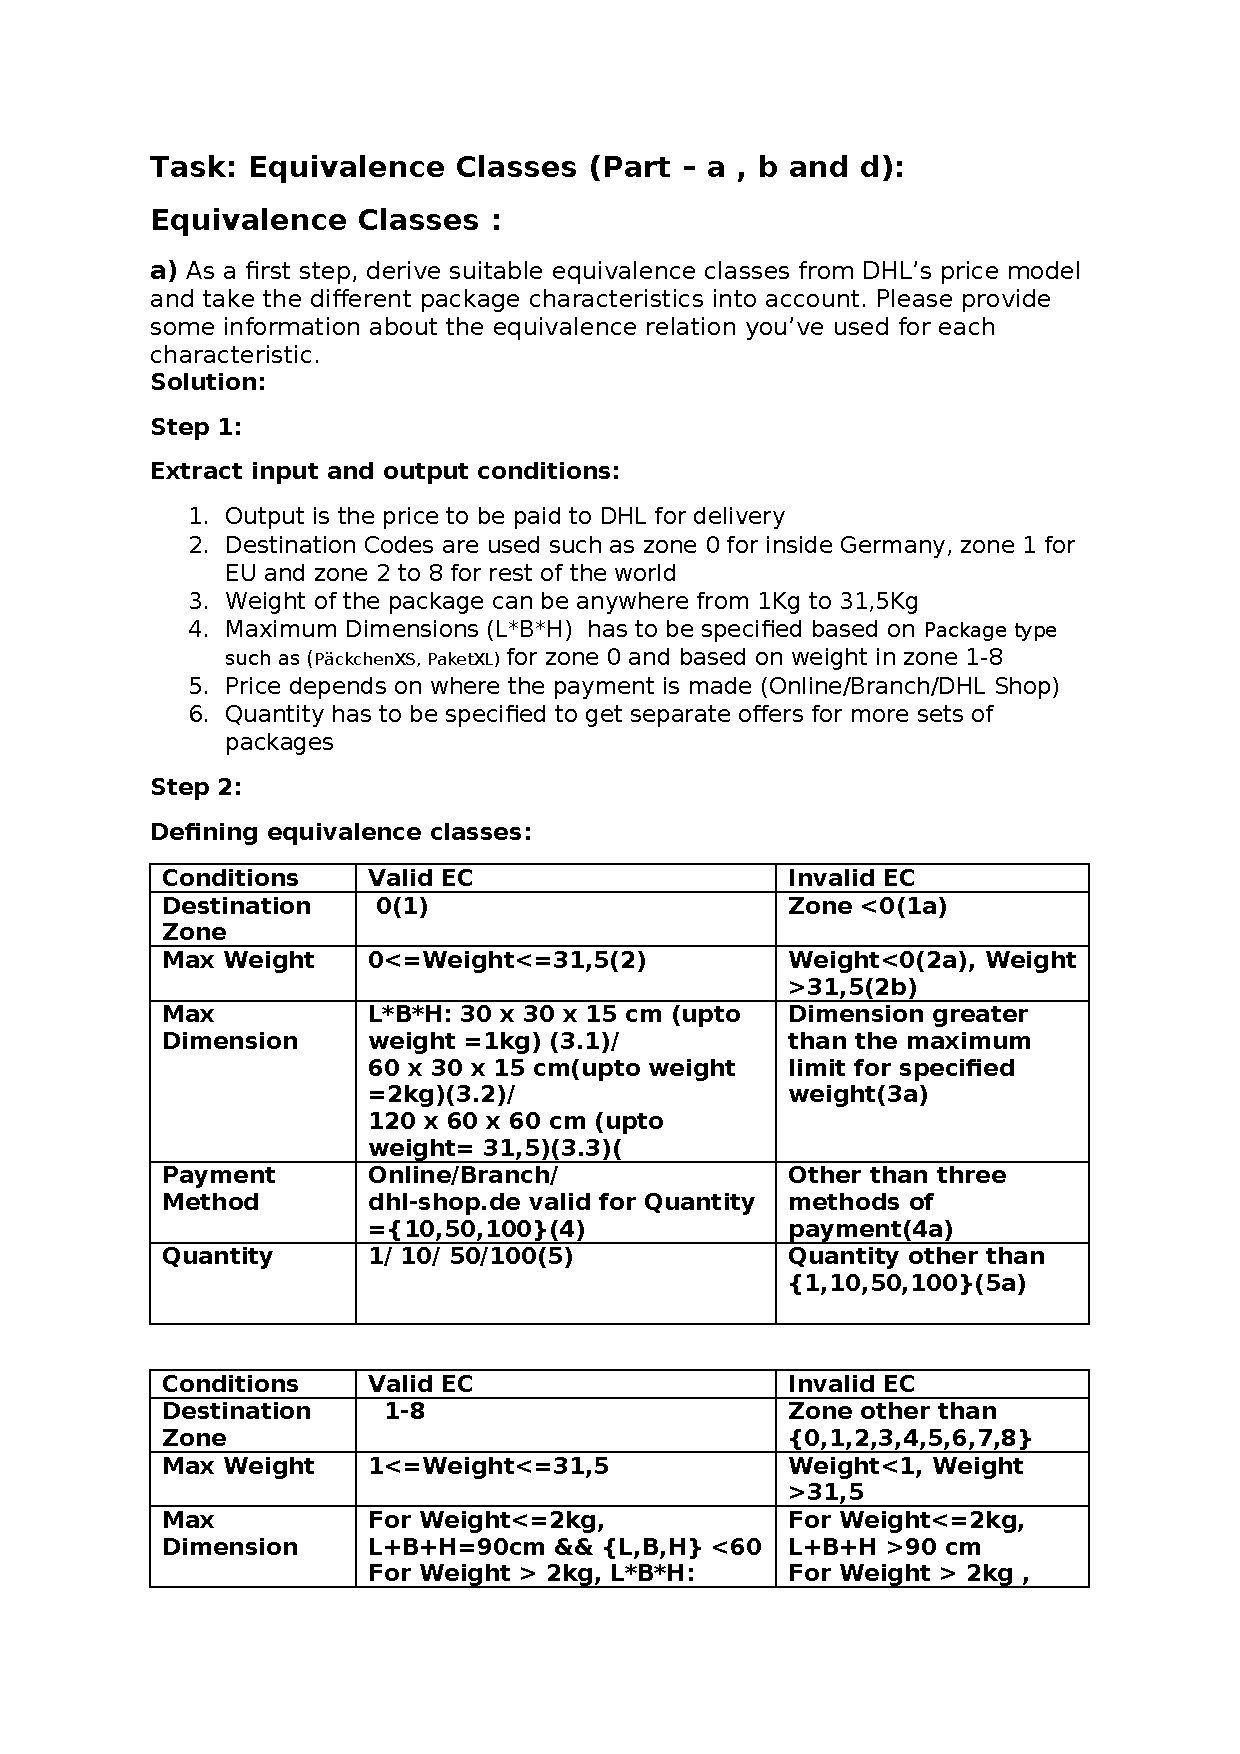
\includegraphics[page=1, clip, trim=1cm 2cm 1cm 2cm, scale=0.90]{others.pdf}
	\clearpage
	\includegraphics[page=2, clip, trim=1cm 2cm 1cm 2cm, scale=0.90]{others.pdf}
	\clearpage
	\includegraphics[page=3, clip, trim=1cm 2cm 1cm 2cm, scale=0.90]{others.pdf}
	\clearpage
	\includegraphics[page=4, clip, trim=1cm 2cm 1cm 2cm, scale=0.90]{others.pdf}
	\clearpage
	\includegraphics[page=5, clip, trim=1cm 2cm 1cm 2cm, scale=0.90]{others.pdf}
	\clearpage
	\includegraphics[page=6, clip, trim=1cm 2cm 1cm 2cm, scale=0.90]{others.pdf}
	\clearpage
	
	\section{Appendix for Task 3.1}
	
\begin{lstlisting}
package de.rwth.swc.teaching.sqa;


import org.apache.commons.lang3.tuple.Triple;
import org.junit.jupiter.api.Assertions;
import org.junit.jupiter.api.BeforeAll;
import org.junit.jupiter.api.DynamicTest;
import org.junit.jupiter.api.Test;
import org.junit.jupiter.api.TestFactory;
import java.util.ArrayList;
import java.util.Arrays;
import java.util.Collection;
import java.util.List;
import java.util.Random;

public class EmailValidatorTest {

	private static EmailValidator validator;
	
	@BeforeAll
	public static void init(){
	validator =  new EmailValidator();
	}
	
	// localPart boundary variables
	public static final int localMinLength_minus = 0;
	public static final int localMinLength = 1;
	public static final int localMinLength_plus = 2;
	
	public static final int localNomLength = 33;
	
	public static final int localMaxLength_minus = 63;
	public static final int localMaxLength = 64;
	public static final int localMaxLength_plus = 65;
	
	// domainPart boundary variables
	public static final int domainMinLength_minus = 0;
	public static final int domainMinLength = 1;
	public static final int domainMinLength_plus = 2;
	
	public static final int domainNomLength = 65;
	
	public static final int domainMaxLength_minus = 127;
	public static final int domainMaxLength = 128;
	public static final int domainMaxLength_plus = 129;
	
	// topLevelPart boundary variables
	public static final int topMinLength_minus = 0;
	public static final int topMinLength = 1;
	public static final int topMinLength_plus = 2;
	
	public static final int topNomLength = 32;
	
	public static final int topMaxLength_minus = 62;
	public static final int topMaxLength = 63;
	public static final int topMaxLength_plus = 64;
	
	String characterPool = new String ("abcdefghijklmnopqrstuvwxyzABCDEFGHIJKLMNOPQRSTUVWXYZ0123456789");
	int characterPoolSize = characterPool.length();
	
	public String stringGeneratorbyLength(Random r, int stringLength) {
		if (stringLength == 0)
			return new String("");
	
		String resultString = new String("");
		for (int i=0; i<stringLength; i++) {
			int pickedValue = r.nextInt(characterPoolSize);
			resultString = resultString + characterPool.charAt(pickedValue);
		}
		
		return resultString;
	}
	
	public Triple<String, String, String> mailGeneratorByLength(Random r, int localLength, int domainLength, int topLength) {
		String _local = stringGeneratorbyLength(r, localLength);
		String _domain = stringGeneratorbyLength(r, domainLength);
		String _top = stringGeneratorbyLength(r, topLength);
		
		Triple<String, String, String> emailTriple = Triple.of(_local, _domain, _top);
		return emailTriple;
	}
	
	
	@TestFactory
	Collection<DynamicTest> simpleBVT() {
		List<Integer> localValues	= Arrays.asList( localMinLength, localMinLength_plus, localMaxLength_minus, localMaxLength);
		List<Integer> domainValues	= Arrays.asList( domainMinLength	, domainMinLength_plus	, domainMaxLength_minus	, domainMaxLength);
		List<Integer> topValues		= Arrays.asList( topMinLength, topMinLength_plus, topMaxLength_minus, topMaxLength);
	
		Random r = new Random();
		ArrayList<DynamicTest> tests = new ArrayList<DynamicTest>();
	
		// all nominal case
		Triple<String, String, String> sNom = mailGeneratorByLength(r, localNomLength, domainNomLength, topNomLength);
		String testMessageNom = "[Simple] -> with [ " + ((Integer)localNomLength) + " " + ((Integer)topNomLength) + " " +  ((Integer)topNomLength) + " ]" ;
		System.out.println(testMessageNom);
		DynamicTest tNom;
		tNom = DynamicTest.dynamicTest(testMessageNom,
		() -> Assertions.assertTrue(validator.validateEMailAdress(sNom.getLeft(), sNom.getMiddle(), sNom.getRight()), "pass"));
		tests.add(tNom);
	
		for (Integer lVal: localValues) 
		{
			Triple<String, String, String> s = mailGeneratorByLength(r, lVal, domainNomLength, topNomLength);
			String testMessage = "[Simple] -> with [ " + lVal.toString() + " " + ((Integer)domainNomLength) + " " + ((Integer)topNomLength) + " ]";
			System.out.println(testMessage);
			DynamicTest t;
			t = DynamicTest.dynamicTest(testMessage,
				() -> Assertions.assertTrue(validator.validateEMailAdress(s.getLeft(), s.getMiddle(), s.getRight()), "pass"));
			tests.add(t);
		}
	
		for (Integer dVal: domainValues) 
		{
			Triple<String, String, String> s = mailGeneratorByLength(r, localNomLength, dVal, topNomLength);
			String testMessage = "[Simple] -> with [ " + ((Integer)localNomLength).toString() + " " + dVal.toString() + " " + ((Integer)topNomLength).toString() + " ]";
			System.out.println(testMessage);
			DynamicTest t;
			t = DynamicTest.dynamicTest(testMessage,
				() -> Assertions.assertTrue(validator.validateEMailAdress(s.getLeft(), s.getMiddle(), s.getRight()), "pass"));
			tests.add(t);
		}
	
		for (Integer tVal: topValues) 
		{
			Triple<String, String, String> s = mailGeneratorByLength(r, localNomLength, domainNomLength, tVal);
			String testMessage = "[Simple] -> with [ " + ((Integer)localNomLength).toString() + " " + ((Integer)topNomLength).toString() + " " + tVal.toString() + " ]" ;
			System.out.println(testMessage);
			DynamicTest t;
			t = DynamicTest.dynamicTest(testMessage,
				() -> Assertions.assertTrue(validator.validateEMailAdress(s.getLeft(), s.getMiddle(), s.getRight()), "pass"));
			tests.add(t);
		}
	
		System.out.println("[Simple] #Cases: " + ((Integer)tests.size()).toString());
		System.out.println();
		return tests;
	}
	
	@TestFactory
		Collection<DynamicTest> robustnessBVT() {
		List<Integer> localValues	= Arrays.asList( localMinLength_minus, localMinLength, localMinLength_plus, localMaxLength_minus, localMaxLength, localMaxLength_plus);
		List<Integer> domainValues	= Arrays.asList( domainMinLength_minus, domainMinLength	, domainMinLength_plus	, domainMaxLength_minus	, domainMaxLength, domainMaxLength_plus);
		List<Integer> topValues		= Arrays.asList( topMinLength_minus, topMinLength, topMinLength_plus, topMaxLength_minus, topMaxLength, topMaxLength_plus);
		
		List<Integer> safeL	= Arrays.asList( localMinLength, localMinLength_plus,localNomLength, localMaxLength_minus, localMaxLength);
		List<Integer> safeD	= Arrays.asList( domainMinLength, domainMinLength_plus, domainNomLength, domainMaxLength_minus	, domainMaxLength);
		List<Integer> safeT	= Arrays.asList( topMinLength, topMinLength_plus, topNomLength, topMaxLength_minus, topMaxLength);
	
		Random r = new Random();
		ArrayList<DynamicTest> tests = new ArrayList<DynamicTest>();
	
		// all nominal case
		Triple<String, String, String> sNom = mailGeneratorByLength(r, localNomLength, domainNomLength, topNomLength);
		String testMessageNom = "[Robustness] -> with [ " + ((Integer)localNomLength) + " " + ((Integer)topNomLength) + " " +  ((Integer)topNomLength) + " ]" ;
		
		Boolean actualResultNom = validator.validateEMailAdress(sNom.getLeft(), sNom.getMiddle(), sNom.getRight());
		Boolean isSafeNom = true;
		System.out.println(testMessageNom + " " + isSafeNom + " | " + actualResultNom);
		
		DynamicTest tNom;
		tNom = DynamicTest.dynamicTest(testMessageNom,
			() -> Assertions.assertTrue(validator.validateEMailAdress(sNom.getLeft(), sNom.getMiddle(), sNom.getRight()), "pass"));
		tests.add(tNom);
	
		for (Integer lVal: localValues) 
		{
			Triple<String, String, String> s = mailGeneratorByLength(r, lVal, domainNomLength, topNomLength);
			Boolean isSafe = safeL.contains(lVal);
			String testMessage = "[Robustness] -> with [ " + lVal.toString() + " " + ((Integer)domainNomLength) + " " + ((Integer)topNomLength) + " ]";
			
			Boolean actualResult = validator.validateEMailAdress(s.getLeft(), s.getMiddle(), s.getRight());
			System.out.println(testMessage + " " + isSafe + " | " + actualResult);
			
			DynamicTest t;
			if (isSafe)
				t = DynamicTest.dynamicTest(testMessage,
					() -> Assertions.assertTrue(validator.validateEMailAdress(s.getLeft(), s.getMiddle(), s.getRight()), "pass"));
			else
				t = DynamicTest.dynamicTest(testMessage,
					() -> Assertions.assertFalse(validator.validateEMailAdress(s.getLeft(), s.getMiddle(), s.getRight()), "pass"));
			tests.add(t);
		}
	
		for (Integer dVal: domainValues) 
		{
			Triple<String, String, String> s = mailGeneratorByLength(r, localNomLength, dVal, topNomLength);
			Boolean isSafe = safeD.contains(dVal);
			String testMessage = "[Robustness] -> with [ " + ((Integer)localNomLength).toString() + " " + dVal.toString() + " " + ((Integer)topNomLength).toString() + " ]";
			
			Boolean actualResult = validator.validateEMailAdress(s.getLeft(), s.getMiddle(), s.getRight());
			System.out.println(testMessage + " " + isSafe + " | " + actualResult);
			
			DynamicTest t;
			if (isSafe)
				t = DynamicTest.dynamicTest(testMessage,
					() -> Assertions.assertTrue(validator.validateEMailAdress(s.getLeft(), s.getMiddle(), s.getRight()), "pass"));
			else
				t = DynamicTest.dynamicTest(testMessage,
					() -> Assertions.assertFalse(validator.validateEMailAdress(s.getLeft(), s.getMiddle(), s.getRight()), "pass"));
			tests.add(t);
		}
	
		for (Integer tVal: topValues) 
		{
			Triple<String, String, String> s = mailGeneratorByLength(r, localNomLength, domainNomLength, tVal);
			Boolean isSafe = safeT.contains(tVal);
			String testMessage = "[Robustness] -> with [ " + ((Integer)localNomLength).toString() + " " + ((Integer)topNomLength).toString() + " " + tVal.toString() + " ]" ;
			
			Boolean actualResult = validator.validateEMailAdress(s.getLeft(), s.getMiddle(), s.getRight());
			System.out.println(testMessage + " " + isSafe + " | " + actualResult);
			
			DynamicTest t;
			if (isSafe)
				t = DynamicTest.dynamicTest(testMessage,
					() -> Assertions.assertTrue(validator.validateEMailAdress(s.getLeft(), s.getMiddle(), s.getRight()), "pass"));
			else
				t = DynamicTest.dynamicTest(testMessage,
					() -> Assertions.assertFalse(validator.validateEMailAdress(s.getLeft(), s.getMiddle(), s.getRight()), "pass"));
			tests.add(t);
		}
		
		System.out.println("[Robustness] #Cases: " + ((Integer)tests.size()).toString());
		System.out.println();
		return tests;
	}
	
	@TestFactory
	Collection<DynamicTest> worstCaseBVT() {
	
		List<Integer> localValues	= Arrays.asList( localMinLength, localMinLength_plus,localNomLength, localMaxLength_minus, localMaxLength);
		List<Integer> domainValues	= Arrays.asList( domainMinLength, domainMinLength_plus, domainNomLength, domainMaxLength_minus	, domainMaxLength);
		List<Integer> topValues		= Arrays.asList( topMinLength, topMinLength_plus, topNomLength, topMaxLength_minus, topMaxLength);
		
		List<Integer> safeL	= Arrays.asList( localMinLength, localMinLength_plus,localNomLength, localMaxLength_minus, localMaxLength);
		List<Integer> safeD	= Arrays.asList( domainMinLength, domainMinLength_plus, domainNomLength, domainMaxLength_minus	, domainMaxLength);
		List<Integer> safeT	= Arrays.asList( topMinLength, topMinLength_plus, topNomLength, topMaxLength_minus, topMaxLength);
	
		Random r = new Random();
		ArrayList<DynamicTest> tests = new ArrayList<DynamicTest>();
	
		for (Integer lVal: localValues) 
		{
			for (Integer dVal: domainValues) 
			{    			
				for (Integer tVal: topValues) 
				{
					Boolean isSafe = (safeL.contains(lVal) && safeD.contains(dVal) && safeT.contains(tVal));
					String testMessage = "[Worst] -> with [ " + lVal.toString() + " " + dVal.toString() + " " + tVal.toString() + " ]";
					
					Triple<String, String, String> s = mailGeneratorByLength(r, lVal, dVal, tVal);
					
					Boolean actualResult = validator.validateEMailAdress(s.getLeft(), s.getMiddle(), s.getRight());
					System.out.println(testMessage + " " + isSafe + " | " + actualResult);
					
					DynamicTest t;
					if ( isSafe )
						t = DynamicTest.dynamicTest(testMessage,
							() -> Assertions.assertTrue(validator.validateEMailAdress(s.getLeft(), s.getMiddle(), s.getRight()), "pass"));
					else
						t = DynamicTest.dynamicTest(testMessage,
							() -> Assertions.assertFalse(validator.validateEMailAdress(s.getLeft(), s.getMiddle(), s.getRight()), "pass"));
					tests.add(t);
				}
			}
		}
		
		System.out.println("[WorstCase] #Cases: " + ((Integer)tests.size()).toString());
		System.out.println();
		return tests;
	}
	
	@TestFactory
	Collection<DynamicTest> robustnessWorstCaseBVT() {
	
		List<Integer> localValues	= Arrays.asList( localMinLength_minus, localMinLength, localMinLength_plus,localNomLength, localMaxLength_minus, localMaxLength, localMaxLength_plus);
		List<Integer> domainValues	= Arrays.asList( domainMinLength_minus, domainMinLength	, domainMinLength_plus, domainNomLength, domainMaxLength_minus	, domainMaxLength, domainMaxLength_plus);
		List<Integer> topValues	= Arrays.asList( topMinLength_minus, topMinLength, topMinLength_plus, topNomLength, topMaxLength_minus, topMaxLength, topMaxLength_plus );
		
		List<Integer> safeL	= Arrays.asList( localMinLength, localMinLength_plus,localNomLength, localMaxLength_minus, localMaxLength);
		List<Integer> safeD	= Arrays.asList( domainMinLength, domainMinLength_plus, domainNomLength, domainMaxLength_minus	, domainMaxLength);
		List<Integer> safeT	= Arrays.asList( topMinLength, topMinLength_plus, topNomLength, topMaxLength_minus, topMaxLength);
	
		Random r = new Random();
		ArrayList<DynamicTest> tests = new ArrayList<DynamicTest>();
	
		for (Integer lVal: localValues) 
		{
			for (Integer dVal: domainValues) 
			{    			
				for (Integer tVal: topValues) 
				{
					Boolean isSafe = (safeL.contains(lVal) && safeD.contains(dVal) && safeT.contains(tVal));
					String testMessage = "[RobustnessWorst] -> with [ " + lVal.toString() + " " + dVal.toString() + " " + tVal.toString() + " ]";
					
					Triple<String, String, String> s = mailGeneratorByLength(r, lVal, dVal, tVal);
					
					Boolean actualResult = validator.validateEMailAdress(s.getLeft(), s.getMiddle(), s.getRight());
					if (isSafe != actualResult)
						System.out.println(testMessage + " " + isSafe + " | " + actualResult);
					
					DynamicTest t;
					if ( isSafe )
						t = DynamicTest.dynamicTest(testMessage,
							() -> Assertions.assertTrue(validator.validateEMailAdress(s.getLeft(), s.getMiddle(), s.getRight()), "pass"));
					else
						t = DynamicTest.dynamicTest(testMessage,
							() -> Assertions.assertFalse(validator.validateEMailAdress(s.getLeft(), s.getMiddle(), s.getRight()), "pass"));
					tests.add(t);
				}
			}
		}
		System.out.println("[RobustnessWorstCase] #Cases: " + ((Integer)tests.size()).toString());
		System.out.println();
		return tests;
	}
}
\end{lstlisting}
\end{document}
